\begin{pastexam}[label={px:ntut-112-ee-ds-07}]{北科大電機所（戊組）112 學年度 第 7 題}
（追蹤）

About graph:
\[
\mathrm{A(G)}=
\begin{array}{c}
\\ v_1\\ v_2\\ v_3\\ v_4\\ v_5\\ v_6\\ v_7
\end{array}
\!\!
\begin{array}{c}
\begin{array}{ccccccc} v_1 & v_2 & v_3 & v_4 & v_5 & v_6 & v_7\end{array}\\
\begin{bmatrix}
0 & 5 & 0 & 0 & 0 & 0 & 9\\
5 & 1 & 3 & 7 & 0 & 0 & 0\\
0 & 3 & 1 & 0 & 0 & 0 & 0\\
0 & 7 & 0 & 0 & 1 & 0 & 2\\
0 & 0 & 0 & 1 & 0 & 1 & 0\\
0 & 0 & 0 & 0 & 1 & 0 & 0\\
9 & 0 & 0 & 2 & 0 & 0 & 0
\end{bmatrix}
\end{array}
\]
(a)A(G) is the adjacency matrix of G. Give the adjacency multi-lists graph representation of the
graph. (5\%)\\
(b)Find minimum spanning tree of the graph via Kruskal's algorithm (start from $v_4$). (5\%)
\end{pastexam}

\begin{pastsoln}
(a) 屬於資結書第~21~章，(b) 屬於第~24~章。

\textbf{先讀出圖}。 矩陣對稱，是無向加權圖，非對角線的非零元素是邊的權重：
$(v_1, v_2)\,5$、$(v_1, v_7)\,9$、$(v_2, v_3)\,3$、$(v_2, v_4)\,7$、$(v_4, v_5)\,1$、$(v_4, v_7)\,2$、$(v_5, v_6)\,1$，共 $7$ 條。
原卷對角線上 $A[v_2][v_2]$、$A[v_3][v_3]$ 是 $1$，字面上是兩個權重 $1$ 的自環；一般講鄰接多重串列和生成樹時，圖都假設
沒有自環，這兩個 $1$ 很可能是筆誤。 下面不把它們當成邊；生成樹本來就不會用到自環（兩端是同一個頂點，Kruskal
一定會跳過），所以 (b) 的答案不受影響。

\begin{center}
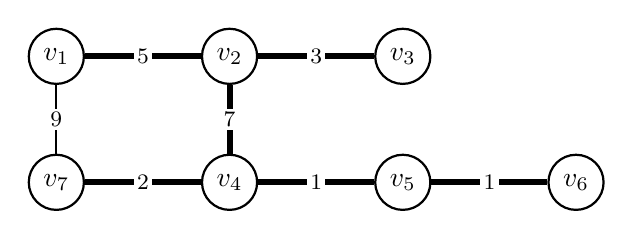
\begin{tikzpicture}[v/.style={circle, draw, thick, minimum size=7mm, inner sep=0pt},
    w/.style={fill=white, inner sep=1.2pt, font=\footnotesize}, e/.style={thick}, t/.style={line width=2.2pt}]
\node[v] (1) at (0,1.6) {$v_1$};
\node[v] (2) at (2.2,1.6) {$v_2$};
\node[v] (3) at (4.4,1.6) {$v_3$};
\node[v] (7) at (0,0) {$v_7$};
\node[v] (4) at (2.2,0) {$v_4$};
\node[v] (5) at (4.4,0) {$v_5$};
\node[v] (6) at (6.6,0) {$v_6$};
\draw[t] (1) -- node[w] {5} (2);
\draw[e] (1) -- node[w] {9} (7);
\draw[t] (2) -- node[w] {3} (3);
\draw[t] (2) -- node[w] {7} (4);
\draw[t] (4) -- node[w] {1} (5);
\draw[t] (4) -- node[w] {2} (7);
\draw[t] (5) -- node[w] {1} (6);
\end{tikzpicture}
\end{center}
（粗線是 (b) 的最小生成樹。）

\textbf{(a)} 鄰接多重串列（資結書第~21.2~節）：每條邊一個節點，欄位是（標記 $m$，兩端 $v_i$、$v_j$，權重，
$\mathit{link}_i$：下一條和 $v_i$ 相關的邊，$\mathit{link}_j$：下一條和 $v_j$ 相關的邊）。 邊依矩陣上三角由上而下、由左而右
編號 $N_1$--$N_7$，每個頂點的邊依編號串起來。

\begin{center}
\small
\begin{tabular}{ccccccc}
\toprule
邊節點 & $m$ & $v_i$ & $v_j$ & 權重 & $\mathit{link}_i$ & $\mathit{link}_j$ \\
\midrule
$N_1$ & 0 & $v_1$ & $v_2$ & 5 & $N_2$ & $N_3$ \\
$N_2$ & 0 & $v_1$ & $v_7$ & 9 & \NIL & $N_6$ \\
$N_3$ & 0 & $v_2$ & $v_3$ & 3 & $N_4$ & \NIL \\
$N_4$ & 0 & $v_2$ & $v_4$ & 7 & \NIL & $N_5$ \\
$N_5$ & 0 & $v_4$ & $v_5$ & 1 & $N_6$ & $N_7$ \\
$N_6$ & 0 & $v_4$ & $v_7$ & 2 & \NIL & \NIL \\
$N_7$ & 0 & $v_5$ & $v_6$ & 1 & \NIL & \NIL \\
\bottomrule
\end{tabular}
\qquad
\begin{tabular}{cc}
\toprule
頂點 & 串列頭 \\
\midrule
$v_1$ & $N_1$ \\
$v_2$ & $N_1$ \\
$v_3$ & $N_3$ \\
$v_4$ & $N_4$ \\
$v_5$ & $N_5$ \\
$v_6$ & $N_7$ \\
$v_7$ & $N_2$ \\
\bottomrule
\end{tabular}
\end{center}
沿著串列走就能列出每個頂點的邊：
$v_1$：$N_1 \to N_2$；$v_2$：$N_1 \to N_3 \to N_4$；$v_3$：$N_3$；$v_4$：$N_4 \to N_5 \to N_6$；$v_5$：$N_5 \to N_7$；
$v_6$：$N_7$；$v_7$：$N_2 \to N_6$。 例如 $v_4$：串列頭 $N_4$，$v_4$ 是 $N_4$ 的 $v_j$ 端，跟 $\mathit{link}_j = N_5$；$v_4$ 是 $N_5$ 的
$v_i$ 端，跟 $\mathit{link}_i = N_6$；$v_4$ 是 $N_6$ 的 $v_i$ 端，$\mathit{link}_i = $ \NIL，結束。 每條邊只存一次，這是它和鄰接串列
（每條邊存兩次）的差別。

\textbf{(b)} Kruskal 演算法（資結書第~24.2~節）是把所有邊依權重由小到大看，兩端不連通就加入，\textbf{沒有起點}；
「start from $v_4$」對 Kruskal 沒有作用（要指定起點的是 Prim）。 照 Kruskal 做：

\begin{center}
\small
\begin{tabular}{clll}
\toprule
邊 & 權重 & 動作 & 加入後的連通塊（只列兩點以上的） \\
\midrule
$(v_4, v_5)$ & 1 & 加入 & $\{v_4, v_5\}$ \\
$(v_5, v_6)$ & 1 & 加入 & $\{v_4, v_5, v_6\}$ \\
$(v_4, v_7)$ & 2 & 加入 & $\{v_4, v_5, v_6, v_7\}$ \\
$(v_2, v_3)$ & 3 & 加入 & $\{v_4, v_5, v_6, v_7\}$、$\{v_2, v_3\}$ \\
$(v_1, v_2)$ & 5 & 加入 & $\{v_4, v_5, v_6, v_7\}$、$\{v_1, v_2, v_3\}$ \\
$(v_2, v_4)$ & 7 & 加入 & $\{v_1, \ldots, v_7\}$ \\
$(v_1, v_7)$ & 9 & 跳過（會成環） & \\
\bottomrule
\end{tabular}
\end{center}
加入 $(v_2, v_4)$ 後已有 $6 = 7 - 1$ 條邊，其實已經可以停；$(v_1, v_7)$ 兩端也已連通。 兩條權重 $1$ 的邊先看哪一條都一樣。 最小生成樹：$(v_4, v_5)$、$(v_5, v_6)$、$(v_4, v_7)$、$(v_2, v_3)$、$(v_1, v_2)$、$(v_2, v_4)$，
總權重 $1 + 1 + 2 + 3 + 5 + 7 = 19$。 圖有 $7$ 條邊，只有 $(v_1, v_7)$ 不在樹上，它是環 $v_1 v_2 v_4 v_7$ 上唯一最重的邊，
所以最小生成樹唯一。

如果出題的意思是「從 $v_4$ 開始做 Prim」：依序加入 $(v_4, v_5)\,1$、$(v_5, v_6)\,1$、$(v_4, v_7)\,2$、$(v_4, v_2)\,7$、
$(v_2, v_3)\,3$、$(v_2, v_1)\,5$，得到同一棵樹。
\end{pastsoln}
